% !TEX root = ../../thesis.tex



\chapter{Introduction} % (fold)

% \textbf{Context:}

Research in humanoid robotics has been thriving in recent years~\parencite{hirai1998development} \parencite{kaneko2008humanoid}, both due to their predicted relevance as personal and assistive robotics~\parencite{tapus2007socially} \parencite{oztop2005human}, and because of the scientific challenges raised by robotics with regards to cognition~\parencite{asada2001cognitive}, natural communication~\parencite{stiefelhagen2004natural} \parencite{breazeal2002robots}, bipedal locomotion~\parencite{yamaguchi1999development} \parencite{chestnutt2005footstep} \parencite{collins2005bipedal} and full-body physical interaction with the environment~\parencite{ude2004programming}.

In the same way as the LHC is an experimental platform for exploring quantum mechanics and the origin of our universe, humanoids can act as simplified and controllable human simulators. Thus humanoid robots can be amazing tools for studying human beings and eventually contribute to a better understanding of human behaviour and abilities~\parencite{atkeson2000using} \parencite{cheng2007cb} \parencite{brooks1986achieving}.

A famous example of such uses of humanoids was the Cog project~\parencite{brooks1999cog} at the Humanoid Robotics Group of the Massachusetts Institute of Technology. This research project had two goals: an engineering goal of building a prototype general-purpose flexible and dextrous autonomous robot and a scientific goal of understanding human cognition~\parencite{brooks1994building}. In particular, this project concentrated on embodiment and interaction intelligence with four aspects of a novel methodology: developmental structure, physical embodiment, integration of multiple sensory and motor systems, and social interaction. For this purpose they built several robotic platform such as a humanoid~\parencite{brooks1999cog} (see \figurename~\ref{fig:brooks_and_cog}), and a very expressive multi-articulated head named Kismet~\parencite{breazeal2003emotion} (see \figurename~\ref{fig:breazeal_kismet}).

% This project ended in 2003 and has brought great scientific contributions such as ... REF


\begin{figure}[t]
\centering
    \subfloat[][Rodney Brooks and the Cog humanoid]{\label{fig:brooks_and_cog}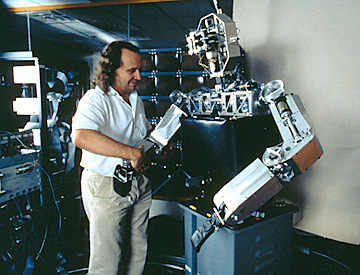
\includegraphics[height=5cm]{brooks_and_cog.jpg}}
    \hfil
    \subfloat[][Cynthia Breazeal with Kismet]{\label{fig:breazeal_kismet}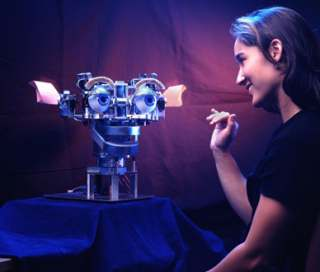
\includegraphics[height=5cm]{breazeal_kismet.jpg}}
    \caption{The Cog project was about the use of computer and robotic technology to better understand and emulate human intelligence.}
    \label{fig:cog_project}
\end{figure}


The context of this PhD thesis is grounded in the same scientific motivations as the work of R. Brooks, R. Pfeifer, T. McGeer and initiative such as the Cog project i.e. \textbf{exploring the role of morphology, cognition and embodiment intelligence in several ways using real experimental robotic platforms}.

The scientific approach of the Cog robots is oriented toward the exploration of embodiment in several ways, from the low level mechatronics to head design for social interactions, but robots were built 15 years ago and using classic manufacturing techniques (see \figurename~\ref{fig:cog_project}) that made them expensive, complicated to modify and especially difficult to diffuse in other laboratories.
We are now in 2014, the makers revolution is in progress~\parencite{anderson2012makers} and novel technologies allow a rethink of the way we design robotic platforms, especially humanoid ones.


In the Inria Flowers team\footnote{\url{flowers.inria.fr}}, we are interested in the study of mechanisms that can allow robots and humans to autonomously and cumulatively acquire repertoires of new skills over extended periods of time. This includes mechanisms for learning by self-exploration, as well as learning through interaction with peers, for the acquisition of both sensorimotor skills (e.g. locomotion, affordance learning and active manipulation) and social skills (e.g. grounded language use and understanding, adaptive interaction protocols, and human-robot collaboration).

With the work An interesting evolution over the last decades has been the demonstration of the importance of robot morphology for sensorimotor control, cognition and development (\parencite{kaplan2008corps} \parencite{steels1995artificial} \parencite{Pfeifer06}). Indeed, robot behaviour cannot be preprogramed. The actual behaviour is always emerging from a complex interaction between the control algorithm, the robot’s morphology and the environment~\parencite{Steels1991emergence}. Moreover, it is clear that a well-adapted robot morphology using specific properties can greatly reduce the complexity of a given task by ensuring implicitly a part -or the entirety- of the control required~\parencite{pfeifer2005morphological}.
Finally, as Rodney Brooks argued, \emph{the world is its own best model}~\parencite{brooks1991intelligence} and simulators cannot realistically handle the complexity of real physics with multi-point contacts, soft material compliance, friction or unpredicted multi-modal interactions.


% \textbf{Needs}

Exploring mechanisms of acquisition requires us to also focus on robot morphology. Therefore, we \textbf{should consider robot morphology\footnote{ robot morphology is defined as any characteristic which defines the physical structure of the robot such as link sizes, number of links, joint characteristics, mass distribution, actuator characteristics, material properties, sensor characteristics and sensor placements~\parencite{paul2006morphological}} as an experimental variable~\parencite{kaplan2008corps} that can be tuned, and conduct experiments in the real world}.

While it is straightforward to explore and experiment with the variation of certain software parameters (e.g. algorithms, simulator), experimenting with morphological variables on a real robot is much more challenging:

\begin{enumerate}
    \item how can we have an experimental robotic platform that allows for morphology to be easily and quickly changed  while acting robustly in the real world?
    \item how can we make this project, mainly the hardware, diffusible and reusable in the research community?
\end{enumerate}

Unfortunately current robotic platforms are not suitable for addressing such challenges.

On one hand, commercial robots such as Nao \parencite{gouaillier2008nao}, Darwin Op \parencite{ha2011development}, Nimbro Op \parencite{schwarznimbro} or iCub \parencite{metta2008icub} are easily accessible and easy to use. Yet they provide a "traditional" morphology (e.g. limited compliance, rigid torso, large feet, over actuation) and modifying their morphology is impractical or impossible. Moreover in most case, they are not open source and/or the hardware is to complicated/expensive to modify.

On the other hand, lab prototypes are mainly handcrafted and specifically tuned which make them almost impossible to reproduce in another lab.

The main issue of these robots is the approaches and technologies chosen to design and produce them. Indeed, the classic way of designing and producing robots is a complicated, time-consuming and expensive process involving specific upfront tooling and complex manufacturing processes.

% \textbf{Task:}

In this thesis, we \textbf{suggest novel approaches and design processes to create and produce robotic platforms,  the control and morphology of which can be freely explored through experimentation in the real world,  that are easy to diffuse and reproduce in the research community.} Especially, this alternative design methodology is driven by the desire to:
\begin{itemize}
    \item freely explore morphological properties,
    \item reduce the amount of time required between an idea and its experimentation on an actual robotic platform in the real world,
    \item makes experiments that should be easy to do, actually easy to do,
    \item make the work easily reproducible in any other lab,
    \item keep the work modular and free to use in accordance with open source principles, so it can be reused and extended for other projects.
\end{itemize}


To reach these goals, we decided to follow novel design methods for both design and production, for all technological aspects of the robot (i.e. mechanics, actuation, electronics, software, distribution). In particular these methods relies on:

\begin{description}
    \item[3D print mechanical parts:] Since few years’ novel techniques, especially 3D printing, are revolutionizing the way we can produce objects. 3D printers open new horizons as they are able to produce parts which were, until now, either not possible or extremely expensive to produce using classical techniques. Especially 3D printing techniques are fast, low-cost and accessible. It allows everyone to produce complex mechanical part in just a couple of hours without requiring any specific upfront tooling.
    These properties of the 3D printing process enable for the first time the exploration of morphological variant for mechanical parts. Indeed, it is now fast and low cost to create alternative design. Associated with modular architecture, we can easily and quickly change robot parts and conduct experiments.
    \item[Electronic architecture based on Arduino] Exploring the role of morphology does not only concern the mechanical properties but also the sensors apparatus i.e. which sensor is used and where it is placed on the body. While it is not yet possible to print complex electronic circuit, we preferred to rely on the Arduino hardware and software environment, which make electronic board easily reconfigurable and compatible with a wide range of sensors. Also, low-level embedded programing skills are not necessary because the board micro-controller can be programmed using Arduino programming language, which abstracts most of the complexity.
    \item[Easy to use python API:] We designed a robust sensory-motor control API adapted to the hardware variability we have. We choose to use Python as it allows fast development, easy deployment on all operating system and quick scripting by non-necessary expert developers. It also offers a large variety of scientific and machine-learning libraries used in robotics (e.g. Numpy, Scipy, Scikit-learn).
    \item[Open source diffusion:] Finally, while the main aspect of such an approach is to allow variability, reuse and modification of the initial design, it is necessary to not only diffuse our work through scientific publications but also to distribute the material needed. This means anyone outside the Flowers lab should have access to the actual source files and be free to make any changes suitable to their own research. Therefore in addition to the technological choices previously presented, we decided to distribute all our work (both software and hardware) under open source licenses. This is an essential step toward building new research tools that facilitate both scientific validation and cumulative science in robotics.

\end{description}

We think this design methodology can contribute to  1) the construction of better experimental robots while making the modification of robot morphology both easy and low cost, and 2) the transfer and reuse of scientific work in other laboratories through the use of open source diffusion.

Within this context we have built a whole new humanoid robot called Poppy\texttrademark (see Fig.~\ref{fig:poppy_with_me}). This humanoid robot was designed to conduct scientific experiments easily and quickly on sensorimotor learning, exploring morphological properties, and human-robot interaction. As an experimental robotic platform, Poppy was designed to be \textbf{affordable}, \textbf{lightweight}, \textbf{robust and safe}, \textbf{easy to use}, \textbf{highly-hackable} and \textbf{fast and easy to duplicate or modify} with the goal of being easily reproducible and used by other labs thanks to an open source distribution (hardware and software).

\begin{figure}[tb]
    \begin{center}
        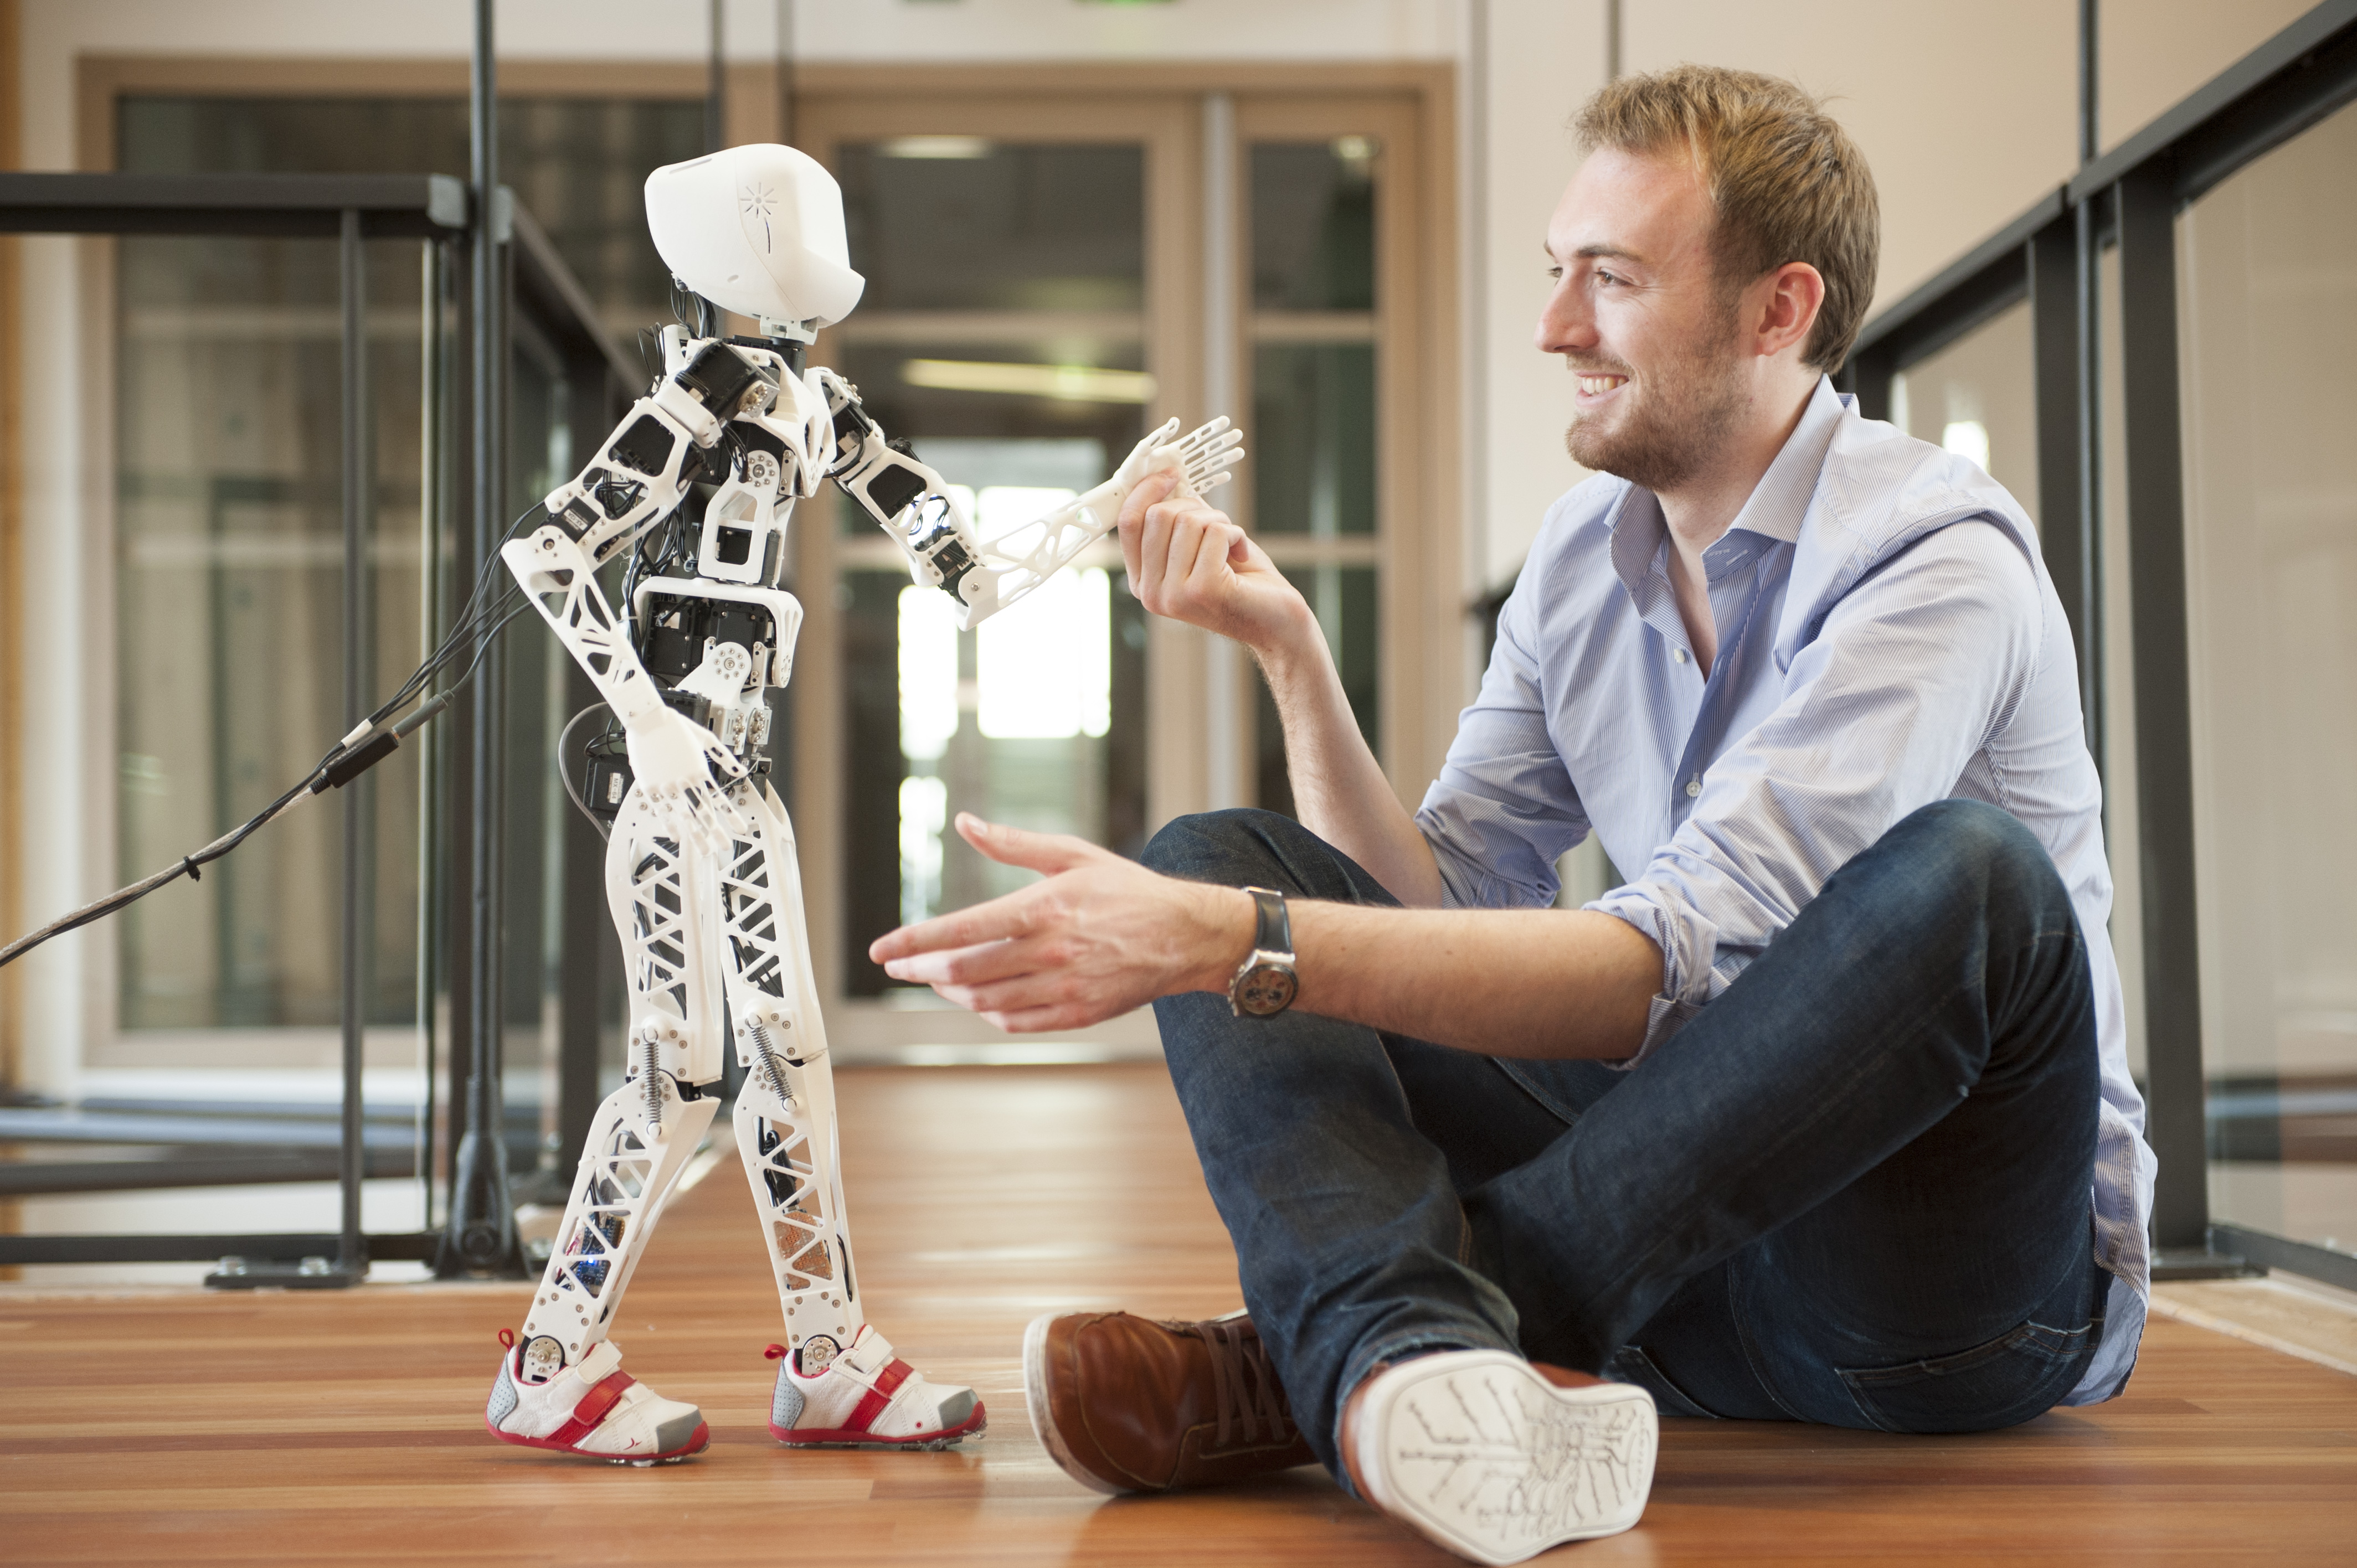
\includegraphics[width=0.7\linewidth]{lapeyre_and_poppy.jpg}
    \end{center}
    \caption{Poppy is a humanoid prototyping platform, which design has been made following the methodology presented in this thesis. It allows for a rich and easy exploration of the robot morphology and its impact on control and cognition. As open source and modular platform, it permits pertinent applications in Science, Art and Education contexts. And is strongly share with open collaboration and cumulative science philosophy}
    \label{fig:poppy_with_me}
\end{figure}

Poppy makes possible exploring new body shapes in just a few days. It enables and simplifies the experimentation, the reproduction and the modification of the morphology in research laboratories. It also allows collaborative working, sharing and replication of the results on these issues between laboratories. The ambition is to become a reference platform for benchmarking and dissemination of scientific results.

Thanks to the fact that it integrates advanced and yet easily accessible techniques in an embodiment that motivates students and the wider public, this platform also meets a growing societal need: education and training in technologies combining computer science, electronics and mechanics, as well as a training tool to the emergent revolutionary 3D printing process. Poppy provides a unique context for experimentation and learning of these technologies in a Do-It-Yourself (DIY) approach. Finally, the possibility to easily modify both the hardware and the software also makes Poppy a useful tool for artistic projects working with interactive computerized installations.


\section*{Proceeding} % (fold)
The proceedings of this thesis will be structured along 4 main parts.

Firstly, a related work will present 1) some inspirational scientific work made over the last 20 years showing the paramount importance of the robot morphology, 2) how we used to design robotic platform until now, and 3) the emergence of the 3D printing techniques and open hardware projects.

We will then describe the development of the Poppy project. In chapter REF we will present the chosen approach to build robotic platform allowing both a free exploration of their morphology and their diffusion in the research community. Then we will present how we used this approach for the design of a novel humanoid platform called Poppy and an easy-to-use robot control library called pypot. We will close this part on the Poppy project's development by the challenges raised by the creation of a research community.

The next part will deal with Poppy's applications and experiments we made about the exploration of morphology (chapter REF) but also for educational (chapter )and artistic (chapter ) purposes.

A discussion part will cloture this thesis. In particular we will discuss potential way to diffuse Poppy and the technological tools we created along this thesis. Following a general discussion of this thesis.

